\section{Code Splitting}
Il code splitting è una particolare implementazione del concetto di Lazy Loading che, in poche parole, consiste nel
dividere il codice JavaScript di grandi dimensioni in frammenti più piccoli chiamati \textbf{chunks}, in modo da
caricare solo ciò che è necessario per il funzionamento di una pagina durante l'avvio rimandando il caricamento degli
altri chunk fino a quando il codice non si rende necessario.  Questo approccio può migliorare notevolmente la reattività
del caricamento della pagina, in quanto riduce il tempo necessario per scaricare e interpretare il codice JavaScript.

\vspace{5mm}
\begin{figure}[H]
    \centering
    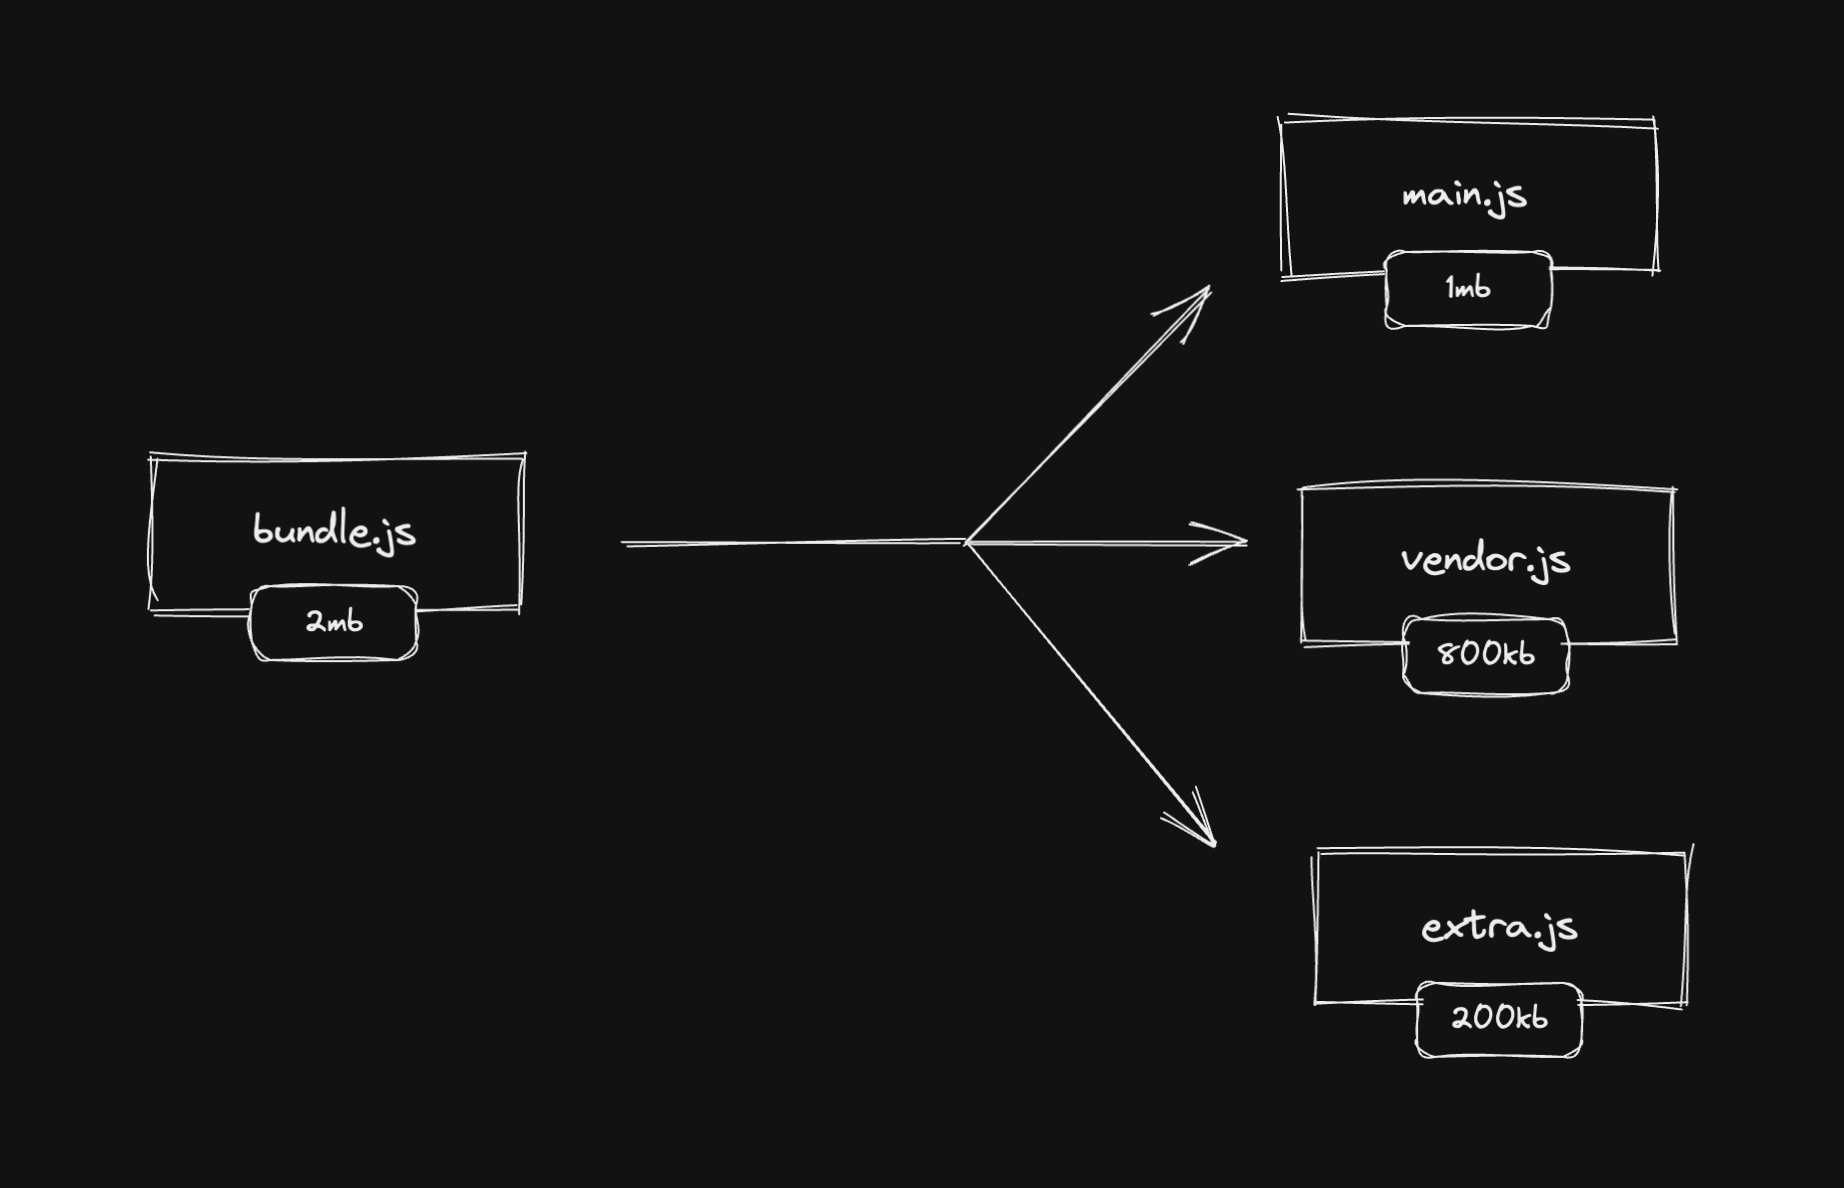
\includegraphics[width=0.8\textwidth]{performance/codesplitting.png}
    \caption{Code Splitting}
\end{figure}

\subsection{Vantaggi e svantaggi del Code Splitting}
Alcuni vantaggi del Code Splitting sono:
\begin{itemize}
    \item \textbf{Caricamento asincrono}: permette di caricare il codice JavaScript in modo asincrono, riducendo il payload iniziale.
    \item \textbf{Riduzione della dimensione del bundle}: riduce la dimensione del bundle JavaScript, migliorando le performance di caricamento.
    \item \textbf{Facilità di implementazione}: è possibile implementare il Code Splitting in modo semplice utilizzando strumenti come Webpack.
\end{itemize}

Di contro, il Code Splitting può comportare alcuni svantaggi:
\begin{itemize}
    \item \textbf{Overhead}: il caricamento asincrono dei chunk può comportare un overhead aggiuntivo.
    \item \textbf{Compatibilità}: alcune funzionalità del Code Splitting potrebbero non essere supportate da tutti i browser.
    \item \textbf{Debugging}: il debugging di applicazioni con Code Splitting può essere più complesso.
    \item \textbf{Cache}: il caching dei chunk può comportare problemi di cache invalidation.
    \item \textbf{Maggior numero di richieste HTTP}: il Code Splitting può comportare un maggior numero di richieste
    HTTP, soprattutto se la dimensione dei chunk è gestita in modo scorretto.
\end{itemize}

